\chapter{Comportamiento de cambio de carril}
\label{ch:lane-change-model}

El problema del cambio de carril determina cuándo y cómo realiza los cambios de carril un conductor en un momento determinado. A priori la intuición sobre el problema es que muchos de los factores determinantes no son medibles en el mundo real y/o en el entorno simulado (e.g. estados de humor, condición física, eventos fortuitos, etcétera).

En un trabajo anterior\cite{CITA DEL ARTÍCULO DE LANE EXECUTION CUANDO NOS LO PUBLIQUEN} se trataron de controlar muchos de estos factores dividiendo el problema en dos partes, la intención de cambio y la ejecución del cambio, fijando el primero de manera que los conductores sólo cambiaban de carril cuando se les ordenaba y permitiendo estudiar, de esta manera, cómo diferentes perfiles de conductores ejecutan de diferente forma el cambio de carril y cómo este fenómenos es modelable.

En este trabajo se tratará de modelar sin embargo el proceso de cambio de carril como un todo, esto es, decidir en cada momento si cambiar a un caril (i.e. izquierda o derecha) o no hacerlo, a partir de las variables medibles del entorno real y simulado.

El problema de ajuste será por tanto un problema de clasificación donde se tratará de maximizar el número de aciertos entre los cambios de carril realizados y el modelo a ajustar. La figura~\ref{fig:lc-lane-change-profiles}.

\begin{figure}
	\centering
	\subfloat[]{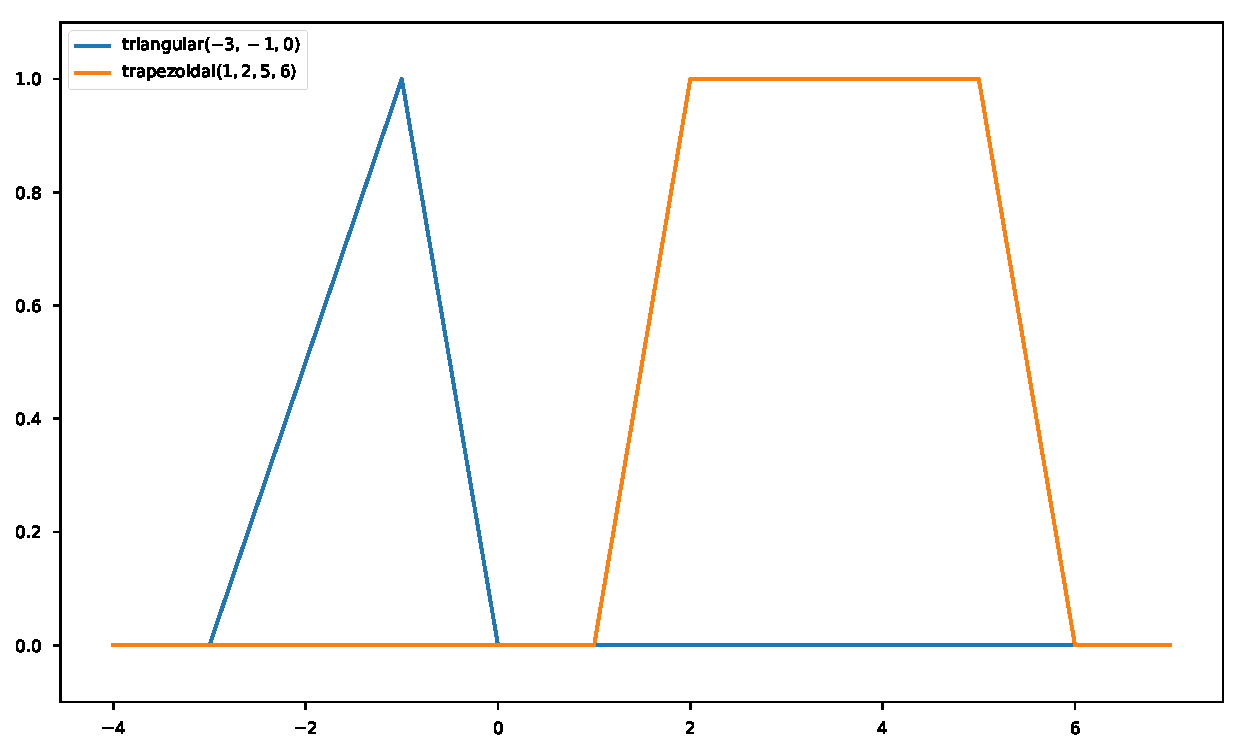
\includegraphics[width=.45\textwidth]{lc-lane-change-hist-training}}\qquad
	\subfloat[]{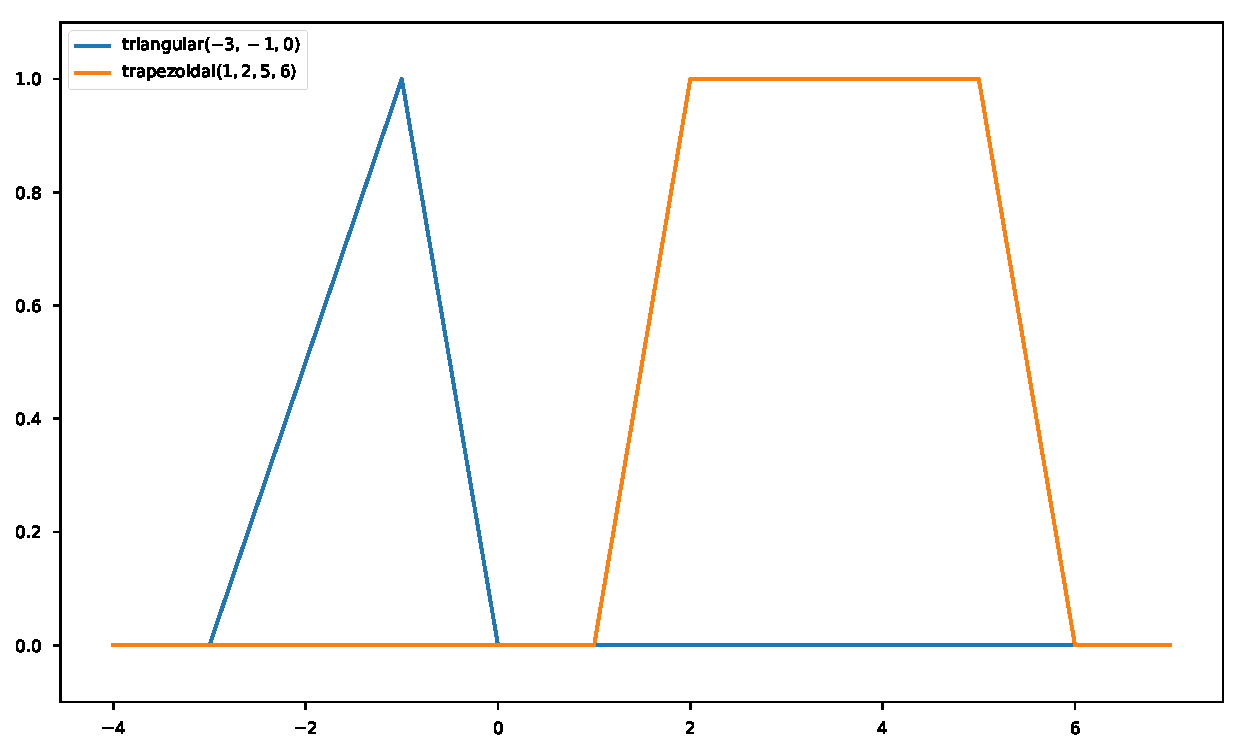
\includegraphics[width=.45\textwidth]{lc-lane-change-hist-test}}
	\caption[Perfiles de cambios de carril en los conjuntos de entrenamiento y test]{Perfiles de cambio de carril en los conjuntos de entrenamiento y de cambios de carril en el conjunto de test. }
	\label{fig:lc-lane-change-profiles}
\end{figure}

Las técnicas que se han seleccionado para tratar el cambio de carril son las siguientes:

\begin{enumerate}
	\item \ac{mlp}. Los \acp{mlp}, más ahora en la época del \textit{deep-learning} son una de las técnicas más usadas para problemas de clasificación. En esta época del \textit{deep-learning} han aumentado su eficiencia varios ordenes de magnitud en capacidad de aprendizaje y, por tanto, en rendimiento a la hora de clasificar.
	\item \ac{cnn}. Otro de los grandes exponentes a la hora de clasificar, sobre todo trabajando con mapas de características $n$-dimensionales con las \acp{cnn}. Al representar la evolución temporal del entorno circundante como un espacio tridimensional, podemos aplicar esta técnica para la identificación de características de manera, supuestamente, más eficiente.
\end{enumerate}

Ambos modelos, al igual que ocurría con el modelo longitudinal, han sido entrenados ajustando sus parámetros con el algoritmo ADAM~\cite{kingma2014adam}. Las funciones de activación, sin embargo, varían, y por tanto la inicialización de las variables también\sidenote{La inicialización clásica, de valores uniformes en un intervalo pequeño alrededor de 0 haría que la mitad de los valores cayesen por debajo de 0. Si la neurona tiene una función de activación de tipo \ac{relu}, el peso no se vería modificado, ya que su derivada será siempre 0}.

En este caso, ambos modelos hacen uso de neuronas de activación de tipo \ac{relu}, salvo en la última capa que la activación es lineal. Para inicializar los pesos de las variables se hace uso del algoritmo Glorot~\cite{glorot2010understanding} (también denominado Xavier) debido a su mejor desempeño, sobre todo en redes con funciones de activación tipo \ac{relu}~\cite{glorot2011deep}\sidenote{Esta inicialización se basa en intentar mantener la misma desviación típica de gradientes en cada capa de la red. En~\cite{glorot2010understanding} determinan que ésta debe ser $\sigma^l = \frac{2}{\mathbf{card}(W^l_{in}) + \mathbf{card}(W^l_{out})}$, siendo $\mathbf{card}(W^l_{in})$ y $\mathbf{card}(W^l_{out})$ el número de entradas y de salidas de la capa, extrayendo posteriormente sus valores de una distribución aleatoria de la forma $X^l \sim \mathcal{N}(\mu=0,\sigma=\sigma^l)$}.

Al tratarse además de un problema de clasificación donde las clases son mutuamente excluyentes, a la capa de salida de las redes se le ha aplicado una normalización\sidenote{
	La normalización usada ha sido la operación denominada softmax, definida como:
	
	\begin{equation}
		softmax(\vec{x})_i = \frac{e^{x_i}}{\sum_{j=1}^n e^{x_j}}
		\label{eq:softmax}
	\end{equation}
} para transformar el vector de salida en un vector de probabilidades, siendo el cambio de carril seleccionado la salida con el valor de probabilidad más alto.

Antes de pasar a la descripción de los modelos, queda hablar del sesgo existente en los datos de entrenamiento. Debido a la naturaleza el problema, el número de ejemplos existentes de cambios de carril es significativamente menor al existente de no cambios de carril. Este sesgo hace que los modelos se entrenen rápidamente para marcar todos los ejemplos como \enquote{no cambio}, dificultando el ajuste posterior hacia cambios a izquierda o derecha.

Por tanto, debido a que (i) las limitaciones de la máquina no nos permiten operar con los conjuntos completos en cada epoch y (ii) existe un sesgo hacia predicciones de \enquote{no cambio}, en cada uno de los epochs, se usará un batch para entrenar de tamaño $m$ compuesto por una selección aleatoria de todos los ejemplos equidistribuida entre las clases de los ejemplos (esto es, aproximadamente $\frac{m}{3}$ para cada clase \enquote{cambio izda.}, \enquote{no cambio} y \enquote{cambio dcha.}).

\section{Modelo \ac{mlp}}

Los entrenamientos han sido realizados sobre diferentes topologías, siendo las más representativas las descritas en la tabla~~\ref{tbl:lc-mlp-architectures}.

\begin{table}
	\caption[Resumen de las arquitecturas \ac{mlp} para el modelo de cambio de carril]{Resumen de las arquitecturas de \ac{mlp} para el modelo de cambio de carril. La posición de cada número de la topología indica la capa, siendo su valor el número de nodos (neuronas) que incluye dicha capa. Las arquitecturas seleccionadas en esta tabla son aquellas consideradas relevantes tras un proceso manual de ensayo y error.}
	\label{tbl:cf-mlp-architectures}
	\begin{tabular}{cccccccccc}
		\hline
		\multirow{2}{*}{Nombre} & \multirow{2}{*}{Topología} & \multirow{2}{*}{Epochs} & \multirow{2}{*}{Dropout} & \multicolumn{3}{c}{Precisión} & \multicolumn{3}{c}{Loss}      \\
		& & & & Training & Validation & Test & Training & Validation & Test \\ \hline
		$MLP_1$ & $X, X, X$ & $10^5$ & $0.1$ & $0.XXX$ & $0.XXX$ & $0.XXX$ & $0.XXX$ & $0.XXX$ & $0.XXX$ \\
		$MLP_2$ & $X, X, X$ & $10^5$ & $0.1$ & $0.XXX$ & $0.XXX$ & $0.XXX$ & $0.XXX$ & $0.XXX$ & $0.XXX$ \\
		$MLP_3$ & $X, X, X$ & $10^5$ & $0.1$ & $0.XXX$ & $0.XXX$ & $0.XXX$ & $0.XXX$ & $0.XXX$ & $0.XXX$ \\
		$MLP_4$ & $X, X, X$ & $10^5$ & $0.1$ & $0.XXX$ & $0.XXX$ & $0.XXX$ & $0.XXX$ & $0.XXX$ & $0.XXX$ \\ \hline
	\end{tabular}
\end{table}

Se han entrenado más redes, pero no se han incluido al no aportar información relevante en la descripción del proceso de entrenamiento.

Cada una de las redes se ha entrenado durante $XXX$ epochs. Debido a las limitaciones de memoria RAM en la máquina de entrenamiento, los epochs no incluyen todo el conjunto de entrenamiento en cada pasada, sino que se limitan a \textit{batches} de $YYY$ elementos seleccionados aleatoriamente del conjunto total de datos.

. En la Figura~\ref{fig:adjusted-fcs} se puede observar la evolución en general y un detalle de la disminución del error en test de los controladores.

\begin{figure}
	\centering
	\subfloat[]{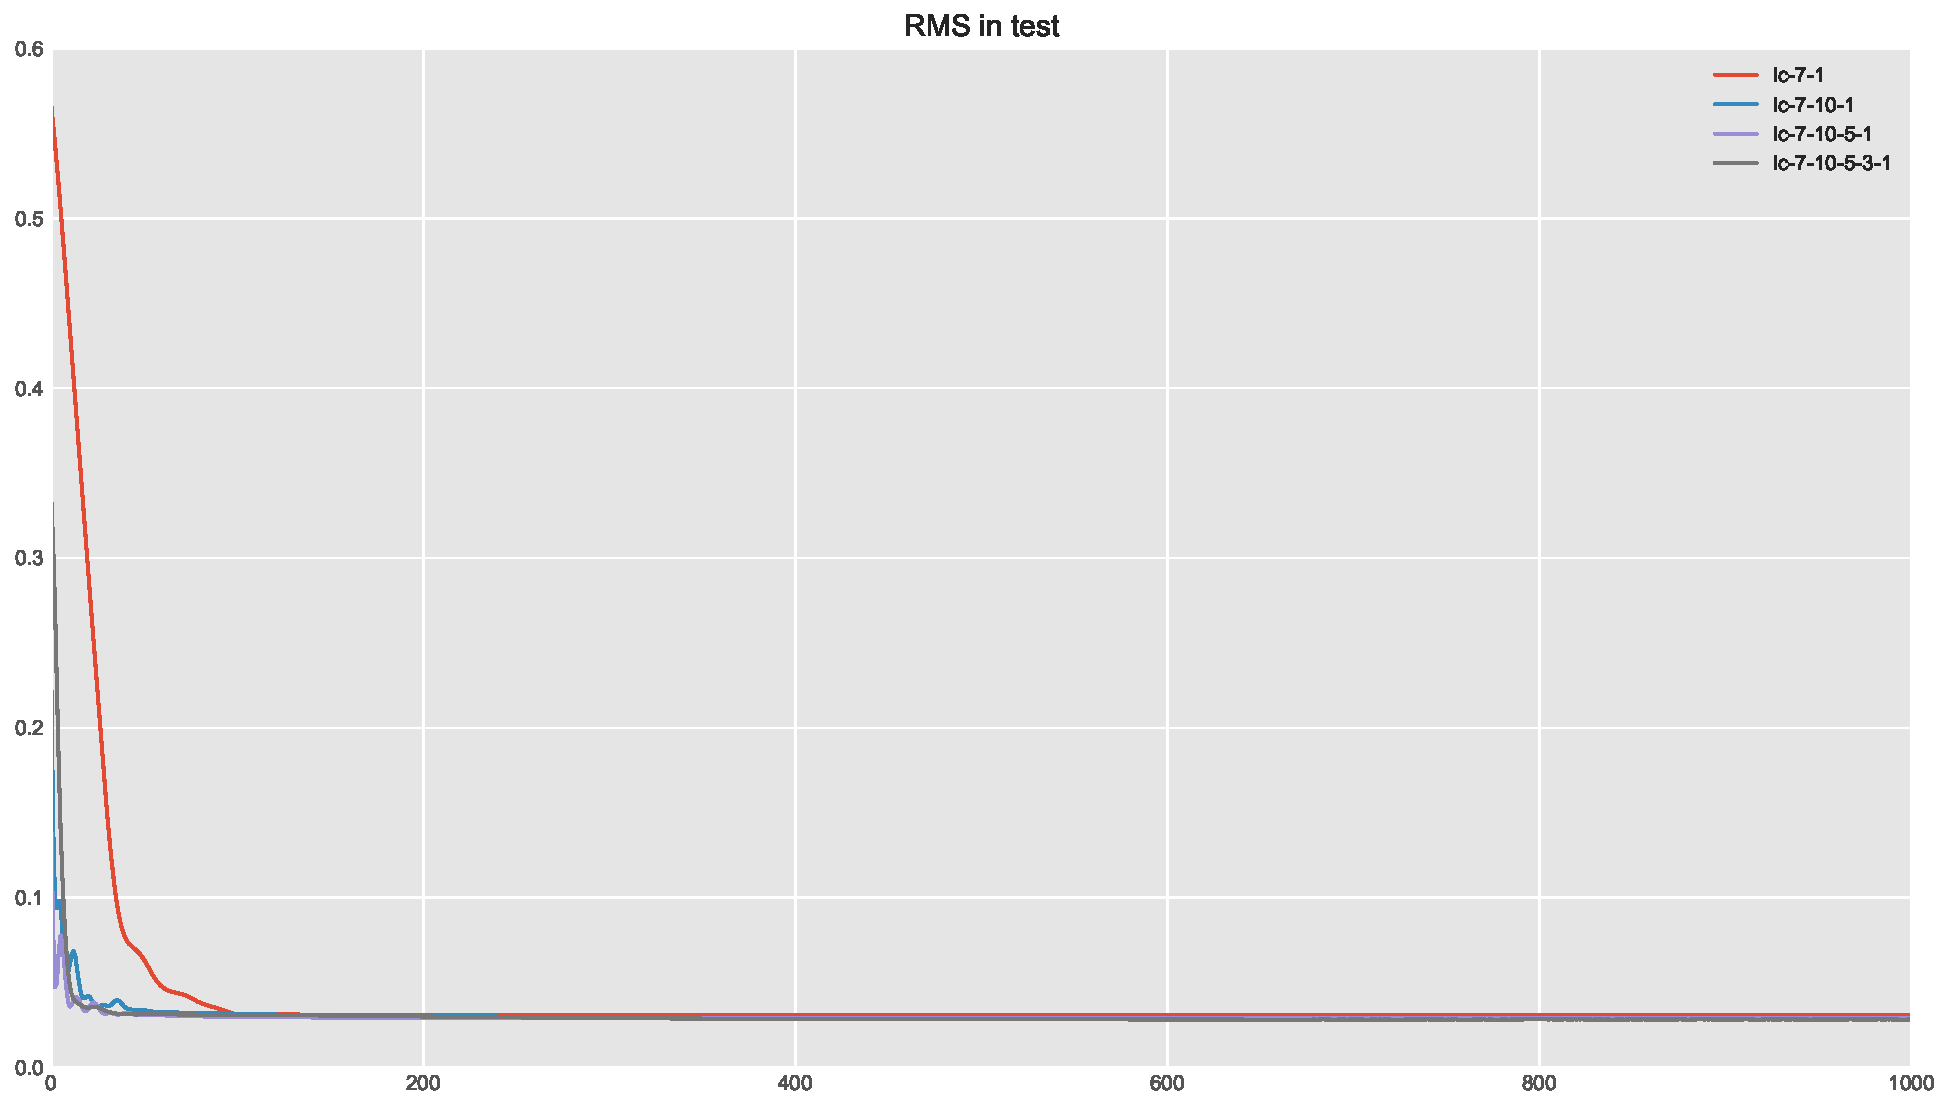
\includegraphics[width=.45\textwidth]{fcs-all-test}}\qquad
	\subfloat[]{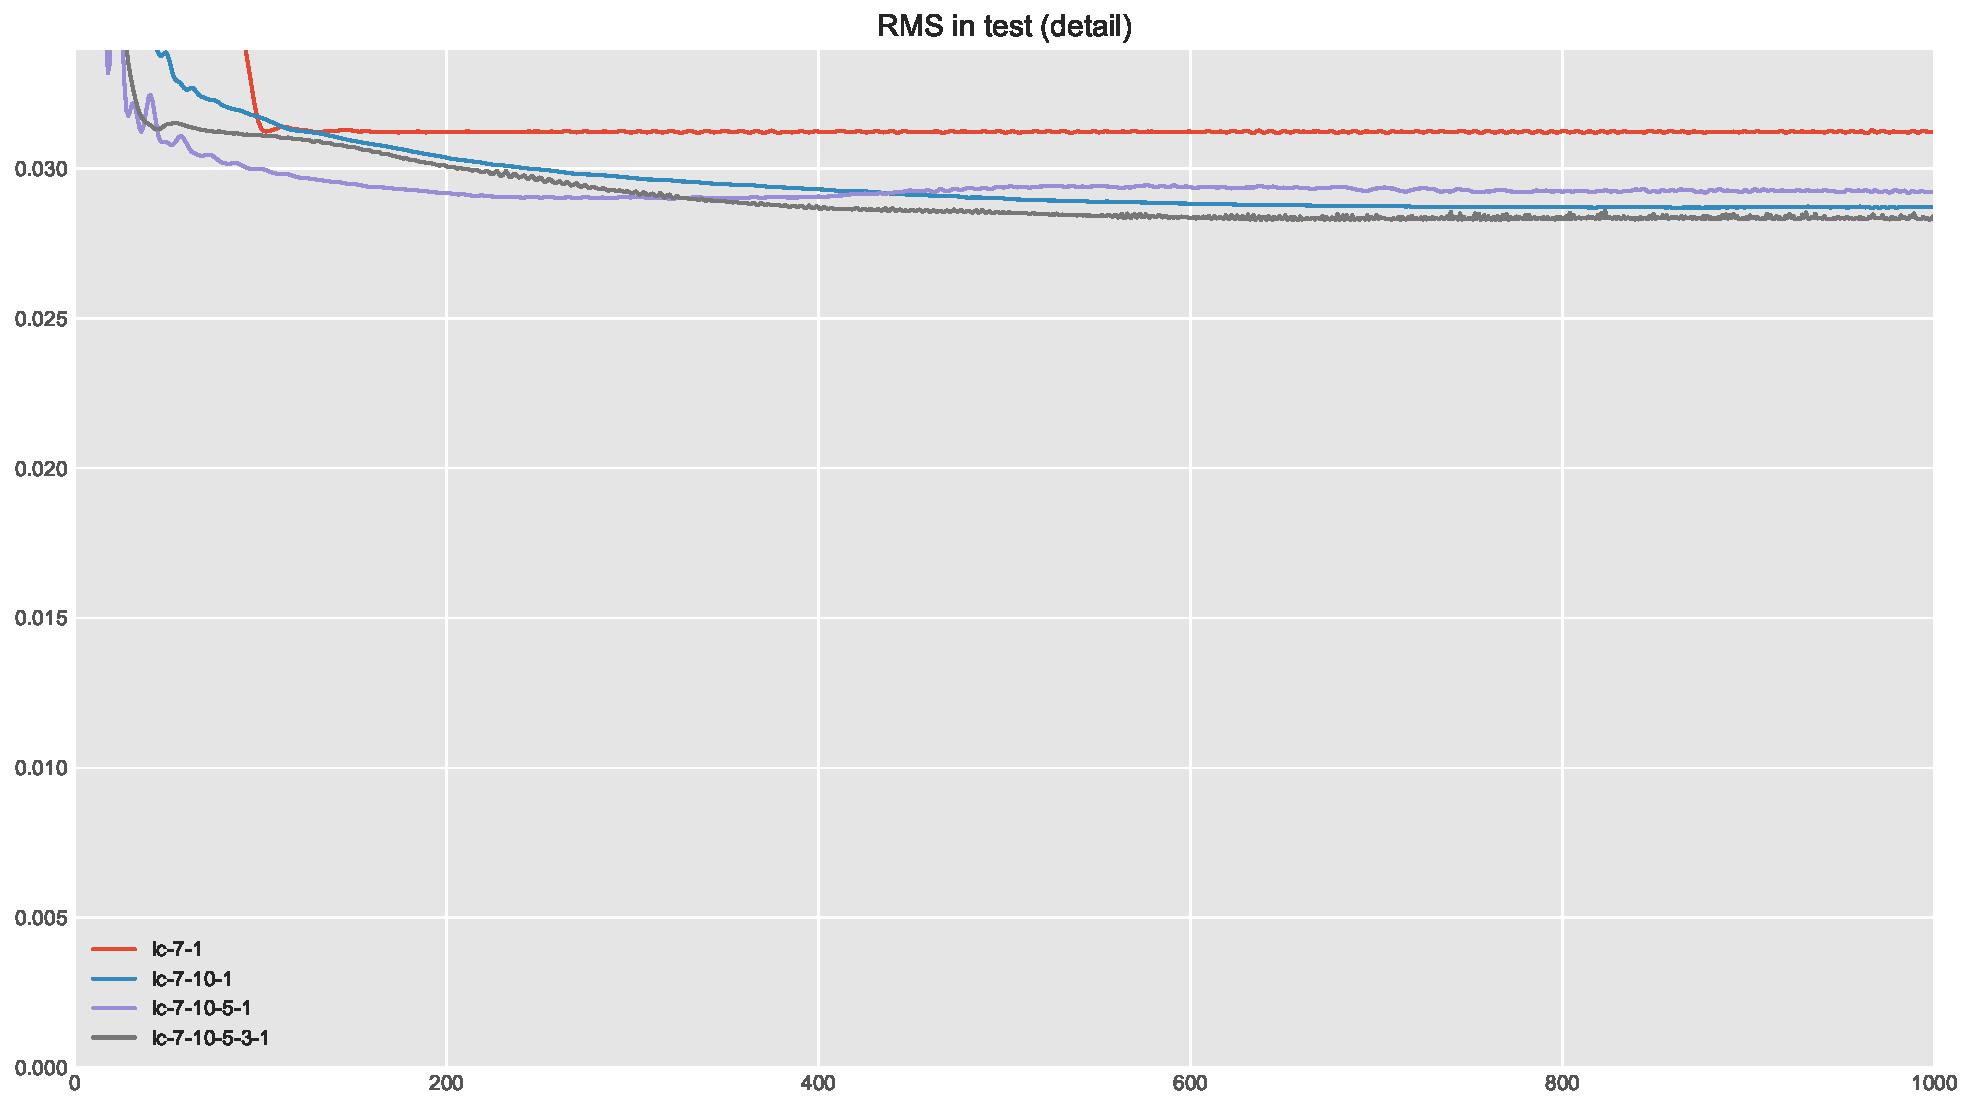
\includegraphics[width=.45\textwidth]{fcs-all-test-detail}}
	\caption[Evolución del error en test de los controladores difusos ajustados]{Visión general y detalle de la evolución del error en test de los diferentes controladores difusos ajustados.}
	\label{fig:adjusted-fcs}
\end{figure}

El proceso de entrenamiento seguido no ha sido el del ajuste de todas las variables en su conjunto. La razón principal de esto es que el ajuste de las variables que determinan las particiones difusas parece suceder órdenes de magnitud más rápido que el ajuste de los pesos asociados a las reglas.

Por tanto, y para este problema en concreto, El entrenamiento se realiza iterativamente alternando conjuntos de epochs dedicados a las reglas y conjuntos de epochs dedicados a las variables de las reglas difusas.

En lugar de eso se ha particionado el entrenamiento en secuencias sucesivas de entrenamiento de reglas y entrenamiento de particiones difusas. Concretamente, los $250.000$ epochs de entrenamiento se corresponden a $250$ iteraciones de $800$ epochs ajustando sólo las reglas seguidos de $200$ epochs ajustando las variables de las particiones difusas.

Empíricamente (y en este problema en concreto) se ha podido observar que el entrenamiento realizado de esta manera hace que el \ac{rmse} descienda más rápido en el mismo número de iteraciones.

Tras el entrenamiento, el controlador difuso que menor error en test arroja es el $FCS_2$\sidenote{
	Para el controlador $FCS_2$, la forma de sus particiones difusas queda, para las variables binarias sin apenas ajuste:
	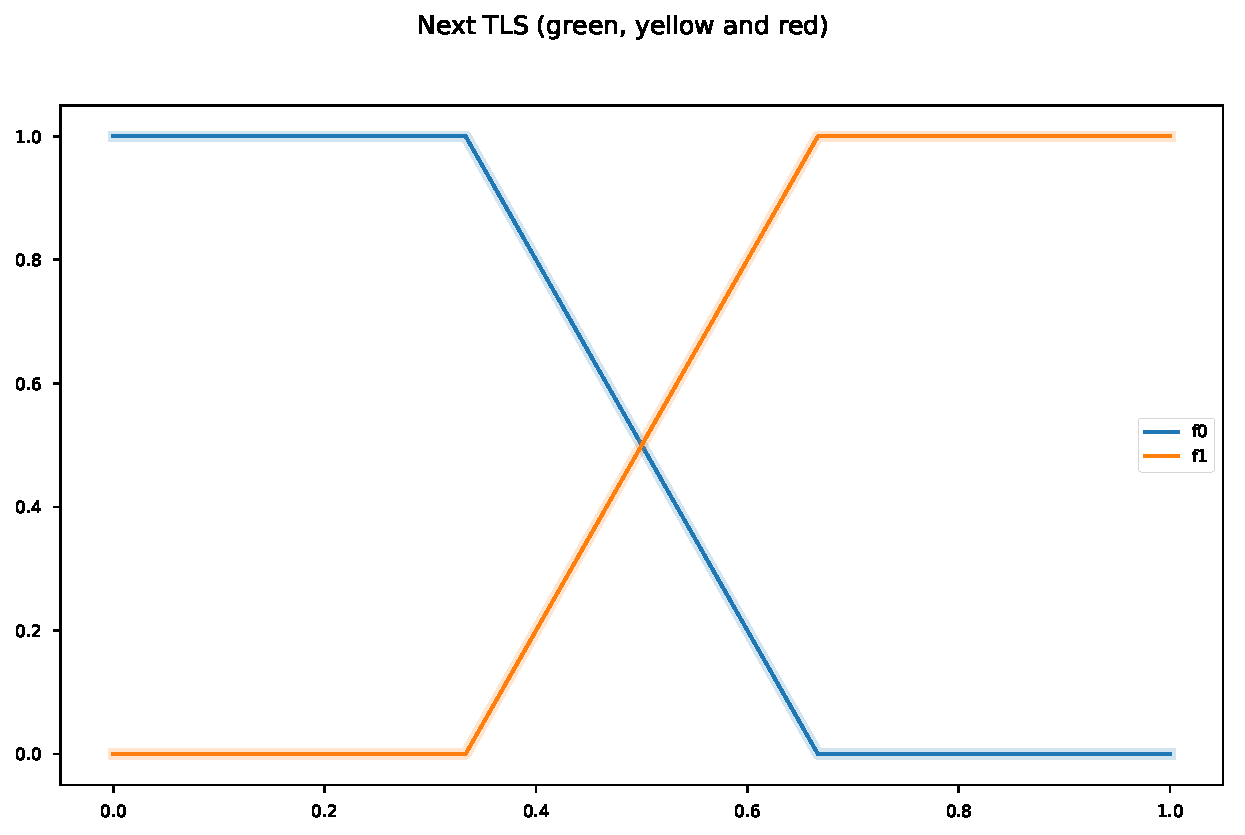
\includegraphics{fcs-best-architecture-next-tls-green-yellow-and-red-variable-partition}
	El resto de particiones sí se han visto modificadas:
	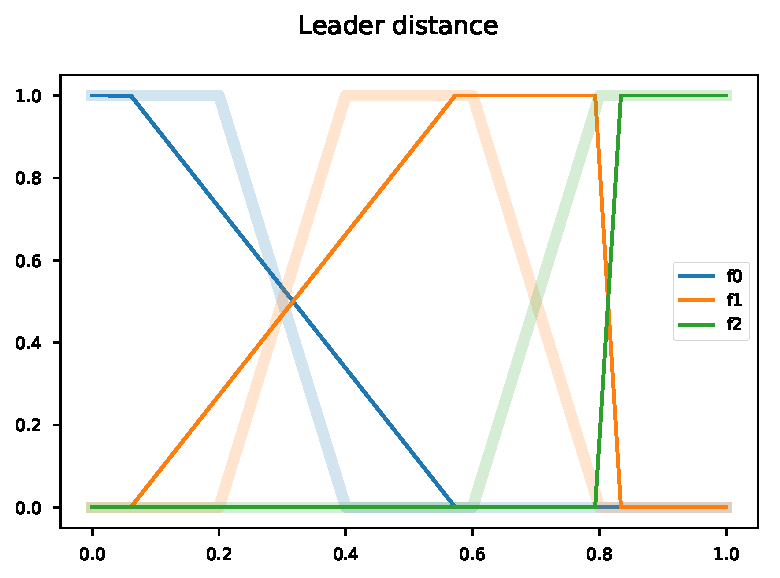
\includegraphics{fcs-best-architecture-leader-distance-variable-partition}
	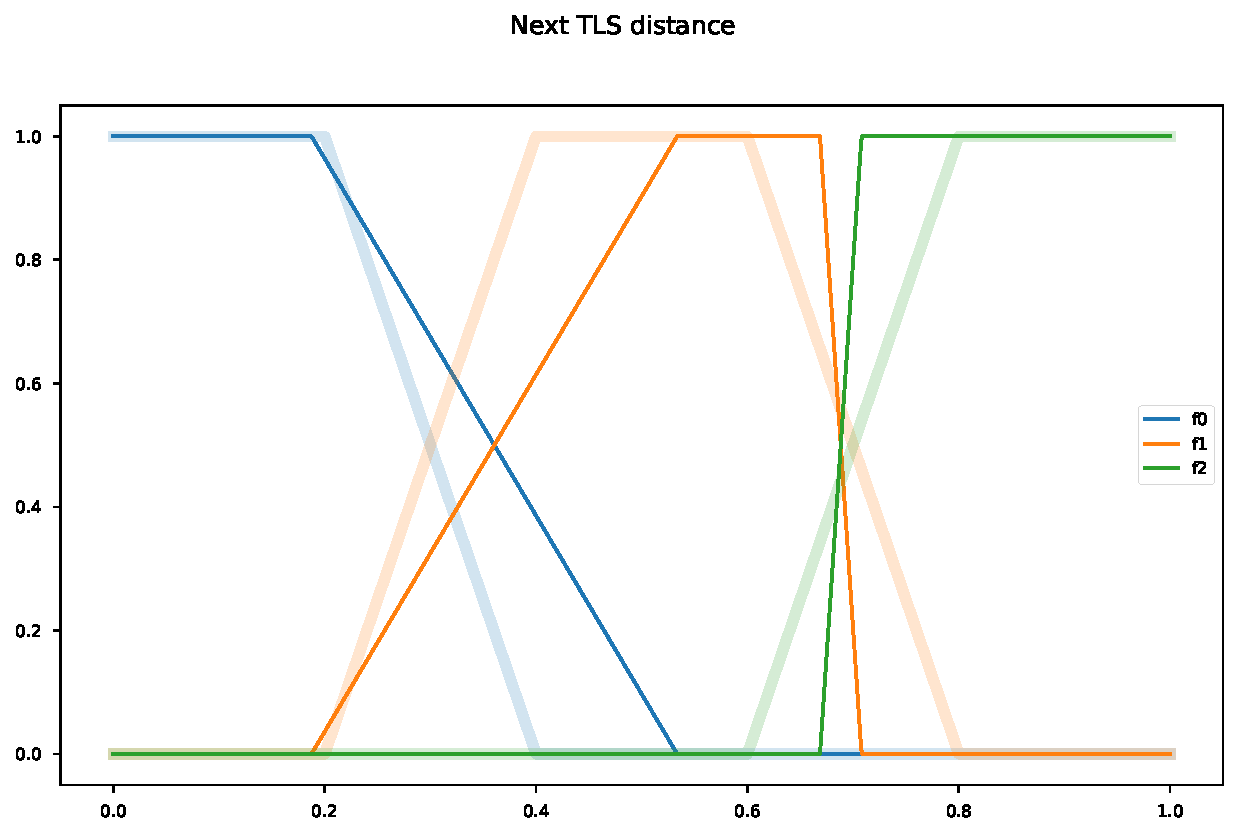
\includegraphics{fcs-best-architecture-next-tls-distance-variable-partition}
	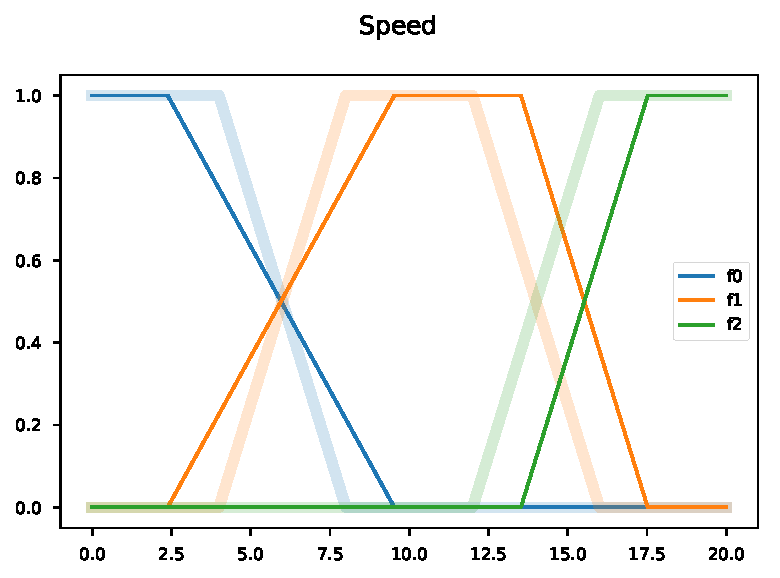
\includegraphics{fcs-best-architecture-speed-variable-partition}
	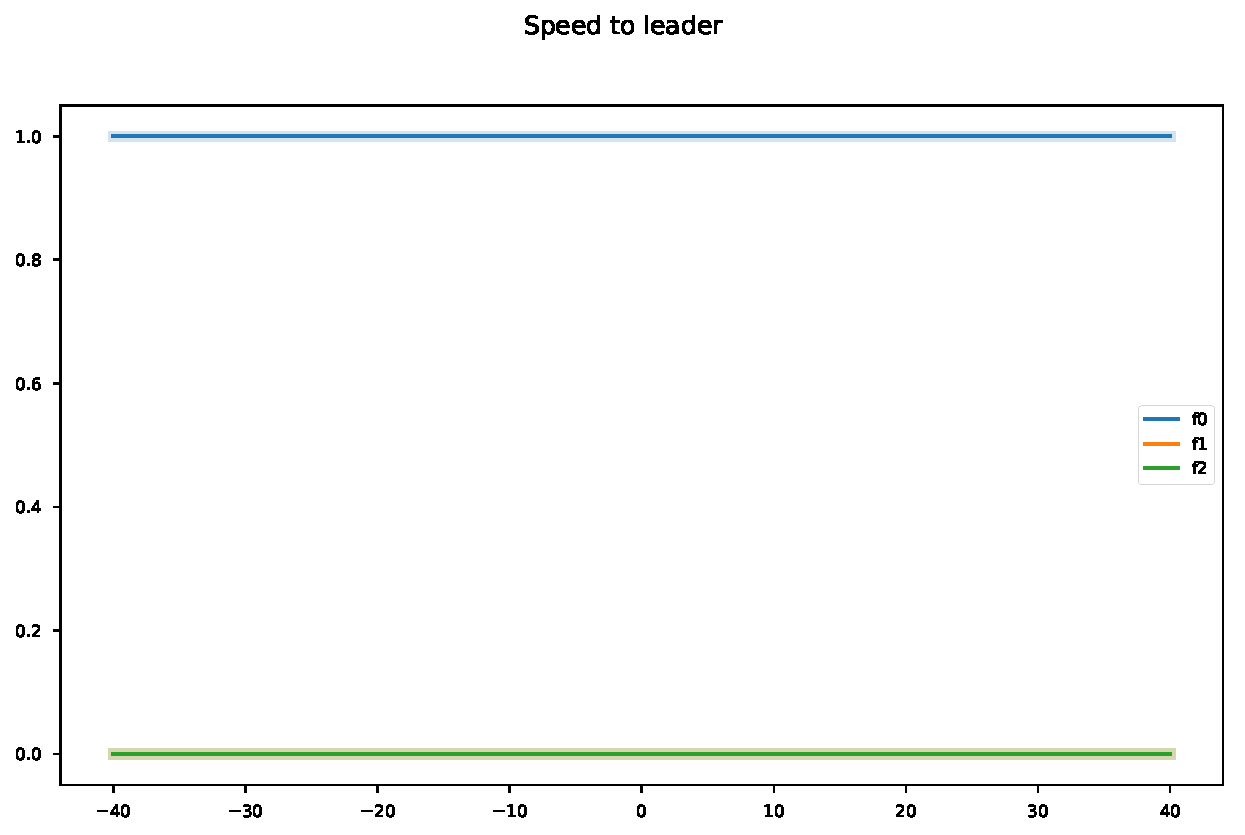
\includegraphics{fcs-best-architecture-speed-to-leader-variable-partition}
	En transparente se puede ver el estado inicial de la partición, y en opaco la forma de ésta tras el proceso de entrenamiento.
}. Por tanto, éste será el modelo seleccionado para la comparativa final.


\section{Modelo \ac{cnn}}

Para determinar el modelo óptimo de \ac{mlp} en comportamiento longitudinal, se han realizado entrenamientos sobre arquitecturas con diferente cantidad de neuronas y capas ocultas. Las arquitecturas más ilustrativas de todas las probadas se resumen en la tabla~\ref{tbl:cf-mlp-architectures}.

\begin{table*}
	\caption[Resumen de las arquitecturas \ac{mlp} para el modelo longitudinal]{Resumen de las arquitecturas de \ac{mlp} para el modelo longitudinal. La posición de cada número de la topología indica la capa, siendo su valor el número de nodos (neuronas) que incluye dicha capa. Las arquitecturas seleccionadas en esta tabla son aquellas consideradas relevantes tras un proceso manual de ensayo y error.}
	\label{tbl:cf-mlp-architectures}
	\begin{tabular}{ccccccc}
		\hline
		\multirow{2}{*}{Nombre} & \multirow{2}{*}{Topología} & \multirow{2}{*}{Epochs} & \multirow{2}{*}{Dropout} & \multicolumn{3}{c}{RMS}      \\
		&                            &                         &                          & Training & Validation & Test \\ \hline
		$MLP_1$ & $7, 16, 1$                 & $10^5$                  & $0.1$                    & $0.052741$      & $0.057301$        & $0.059253$  \\
		$MLP_2$ & $7, 8, 4, 1$               & $10^5$                  & $0.1$                    & $0.056341$      & $0.061951$        & $0.056607$  \\
		$MLP_3$ & $7, 16, 8, 1$              & $10^5$                  & $0.1$                    & $0.046404$      & $0.051878$        & $0.059681$  \\
		$MLP_4$ & $7, 16, 16, 8, 1$          & $10^5$                  & $0.1$                    & $0.042789$      & $0.046876$        & $0.060971$  \\ \hline
	\end{tabular}
\end{table*}

El modelo de neuronas de activación que se ha utilizado es de tipo tangente hiperbólica en todas las neuronas salvo en la última, que se ha utilizado una activación lineal en todas las neuronas salvo en la neurona de salida que se ha utilizado una activación lineal\sidenote{Se han utilizado también funciones de activación de tipo \ac{relu}, pero las tasas de error tras el entrenamiento eran notablemente más altas por lo que se ha optado al final por el uso de activación basada en tangente hiperbólica.}. Los pesos de la red han sido inicializados con una muestra aleatoria uniforme de valores reales en el intervalo $(-0.25, 0.25)$.

El error que se trata de minimizar es el error cuadrático medio entre los valores de aceleración del conjunto reales y los ajustados por el modelo. La Figura~\ref{fig:rms-all-in-training-and-validation-mlp-detail} muestra la evolución de este error durante el proceso de entrenamiento.

\begin{figure}
	\centering
	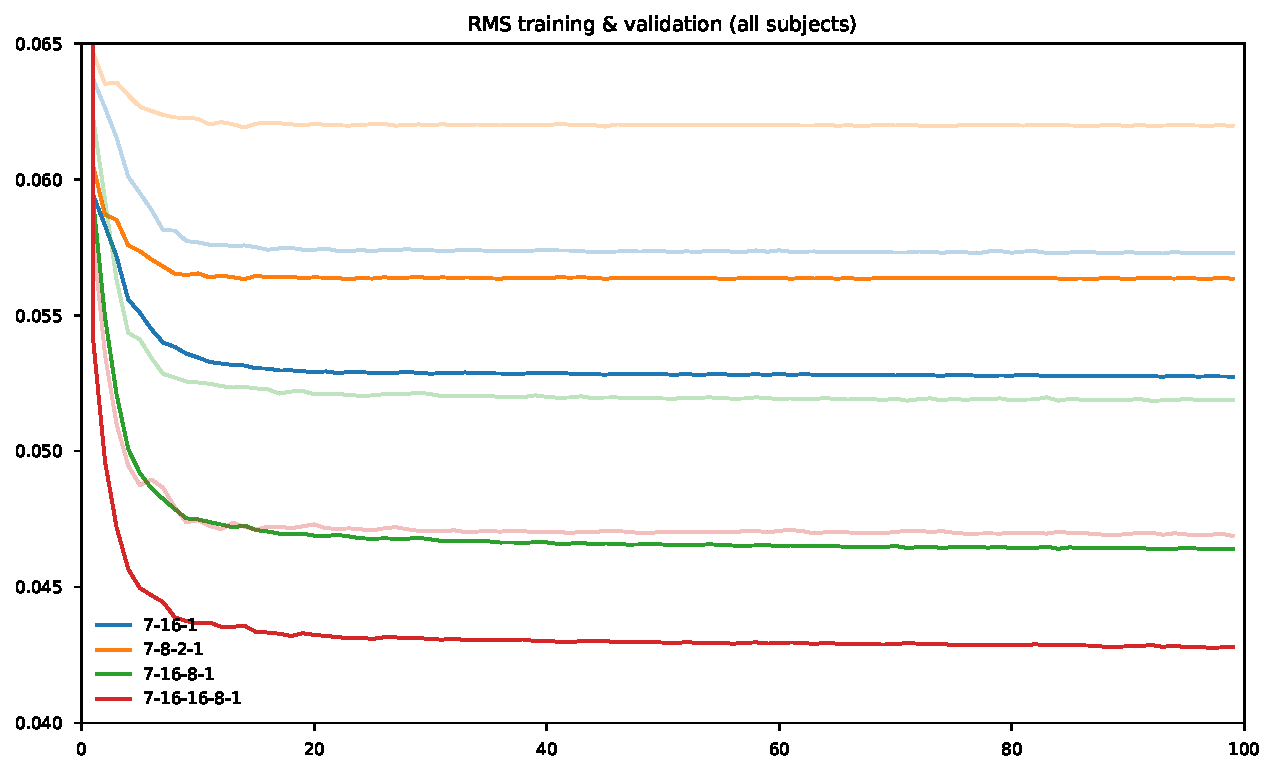
\includegraphics{rms-all-in-training-and-validation-mlp-detail}
	\caption[Evolución del error en entrenamiento en los \ac{mlp} para las arquitecturas seleccionadas]{Visión en detalle de la evolución del error en los conjuntos de entrenamiento y validación. Para cada arquitectura, el color más transparente se corresponde al error en el conjunto de validación..}
	\label{fig:rms-all-in-training-and-validation-mlp-detail}
\end{figure}

Estos errores se encuentran entre los \SI{0.05}{\metre\per\square\second} y los \SI{0.07}{\metre\per\square\second}, lo cual consideramos que es una aproximación aceptable. Una particularidad del problema ha sido la inestabilidad de los entrenamientos, esto es, la alta sensibilidad a los valores de inicialización de los parámetros. La intuición tras ver la evolución de los entrenamientos es que la función de error del problema tiene muchos mínimos locales o mesetas.

Al contrastar los errores de test, podemos determinar que la arquitectura que parece que mejor generaliza es la $MLP_2$ (arquitectura $7, 8, 2, 1$), como podemos ver en la figura~\ref{fig:rms-all-test-mlp-detail}.

\begin{figure}
	\centering
	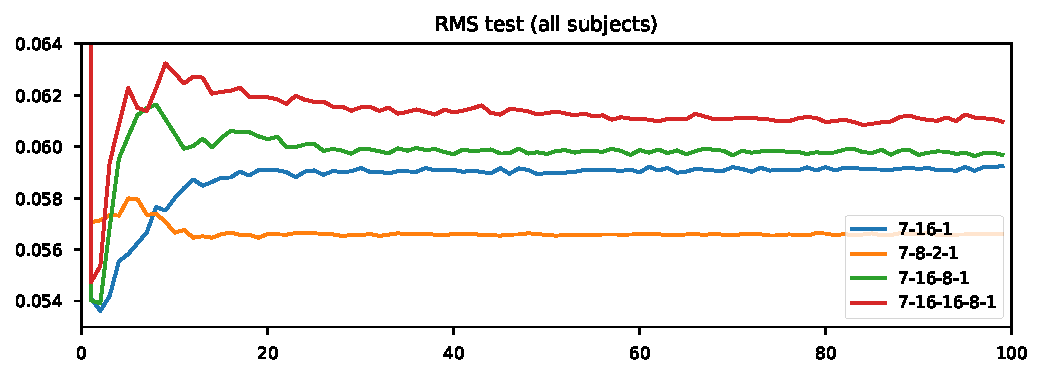
\includegraphics{rms-all-test-mlp-detail}
	\caption[Evolución del error en el conjunto de test durante el entrenamiento]{Visión en detalle de la evolución del error en el conjunto de test. Aunque no se ha considerado para determinar las arquitecturas, sí se ha recogido la información de la evolución del error en el conjunto de test debido a que nos ofrece puede ofrecer intuición de qué forma aprende la red. Por lo que podemos observar, para el problema en cuestión las redes más potentes tienden a sobre-entrenarse.}
	\label{fig:rms-all-test-mlp-detail}
\end{figure}

Una visión de detalle del ajuste de estas arquitecturas al conjunto de test se puede ver en la figura~\ref{fig:mlp-test-comparisons}, donde se muestra el perfil de aceleración del conjunto de test y los perfiles de aceleración de las redes entrenadas.

\begin{figure}
	\centering
	\subfloat[]{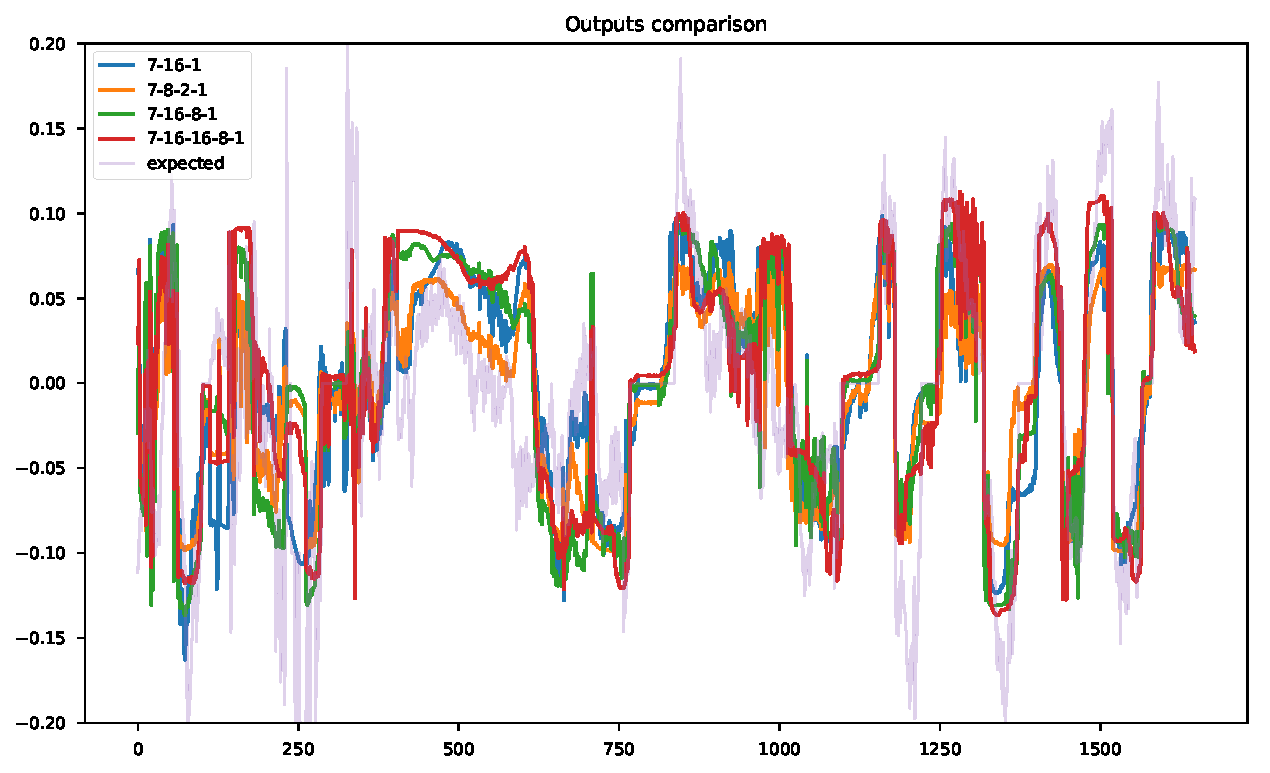
\includegraphics[width=.45\textwidth]{mlp-test-comparison}}\qquad
	\subfloat[]{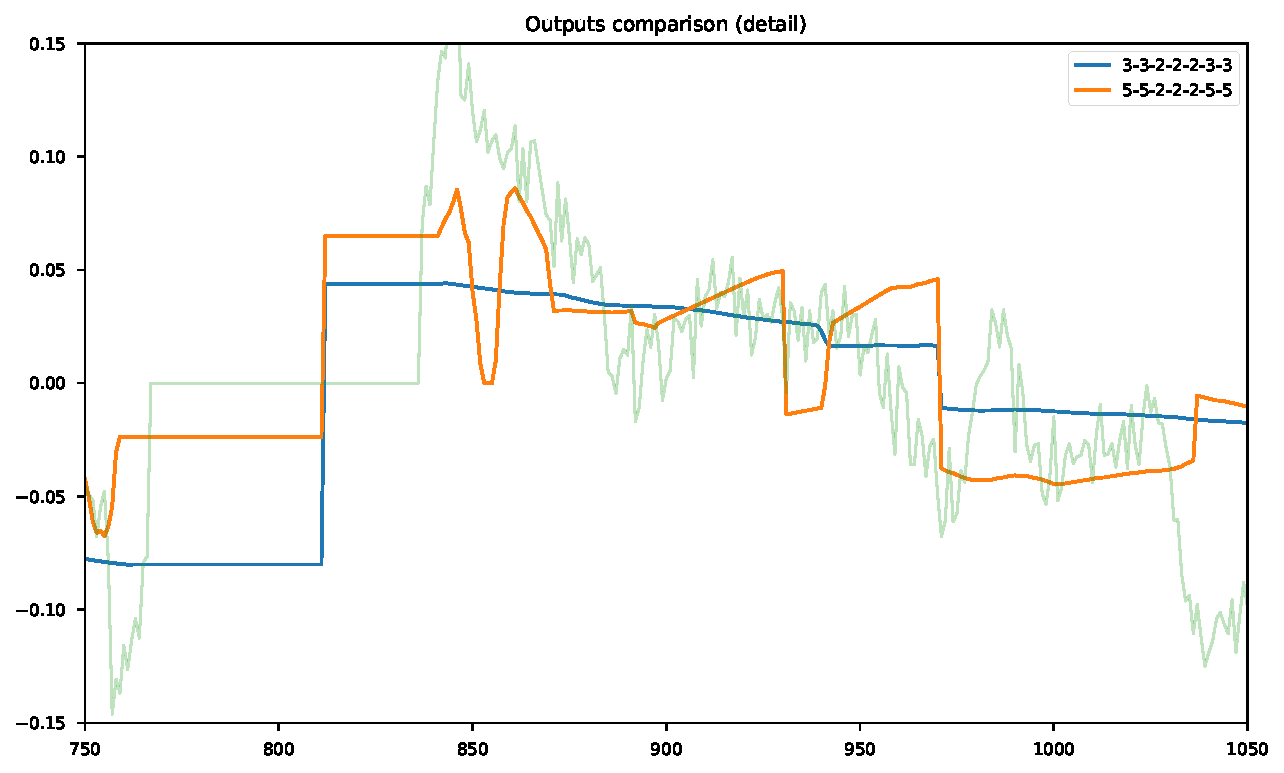
\includegraphics[width=.45\textwidth]{mlp-test-comparison-detail}}
	\caption[Comparación del perfil de aceleración real y el inferido por los modelos entrenados]{Comparación del perfil de aceleración real y el inferido por los modelos entrenados. En la visión general se puede observar, en transparente, el perfil real. A la derecha se amplía una pequeña sección del perfil para mostrar los diferentes ajustes de los modelos entrenados y cómo difieren del valor real.}
	\label{fig:mlp-test-comparisons}
\end{figure}

A la vista de los resultados, y dado que las arquitecturas se ajustan razonablemente bien, es razonable elegir el modelo $MLP_2$ debido a que es el que aparentemente mejor generaliza los comportamientos del conjunto de conductores.

\section{Comparación entre modelos}

Las mejores arquitecturas de ambos modelos han sido la $MLP_2$ para los \acp{mlp} y $FCS_x$ para los \acp{fcs}. Los errores y el perfil de aceleración para ambos modelos se muestran en la figura~\ref{fig:comparison-between-best-mlp-and-fcs-architecture}.

\begin{figure}
	\centering
	\subfloat[]{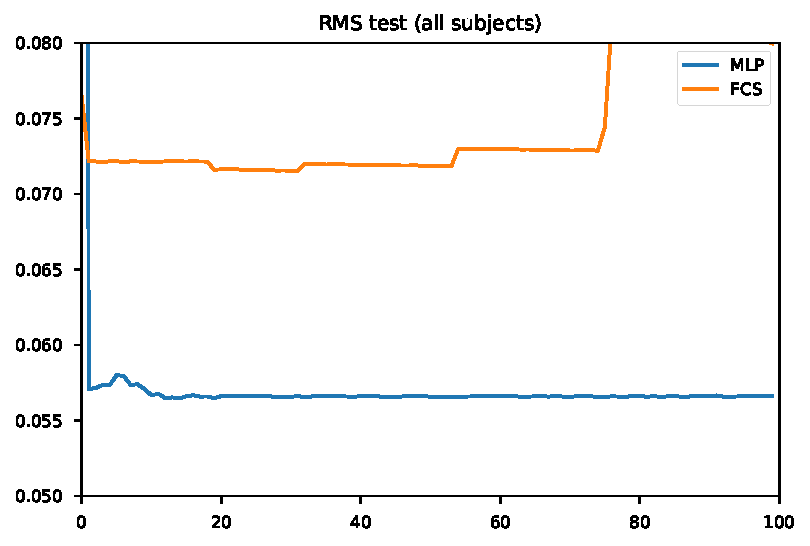
\includegraphics[width=.46\textwidth]{comparison-between-best-mlp-and-fcs-architecture-rms}}\qquad
	\subfloat[]{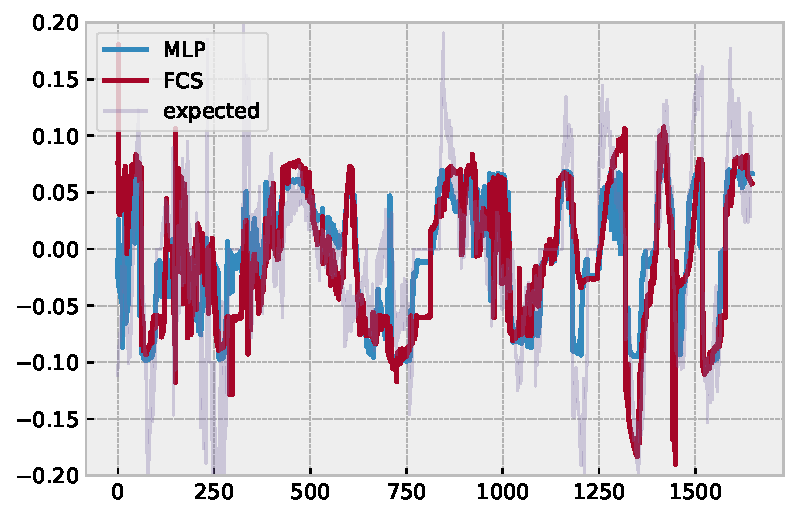
\includegraphics[width=.46\textwidth]{comparison-between-best-mlp-and-fcs-architecture-acceleration-profile}}
	\caption[Comparación entre los dos tipos de modelo longitudinal]{Comparación de la mejor arquitectura \ac{mlp} frente a la mejor arquitectura \ac{fcs}: (a) diferencia entre los errores cuadráticos medios de ambas arquitecturas y (b) perfiles de aceleración en el conjunto de test.}
	\label{fig:comparison-between-best-mlp-and-fcs-architecture}
\end{figure}

Aunque el modelo basado en \ac{fcs} arroja un error bajo en test y parece que tiende a ajustarse al perfil de aceleración, parece que el problema es suficientemente complejo como para no poder representarse como un simple controlador difuso.

Además, el error arrojado por el \ac{mlp} es sustancialmente menor y, por tanto, la arquitectura elegida para el modelo longitudinal será el \ac{mlp} $MLP_2$.